\begin{figure}[H]
  \centering
  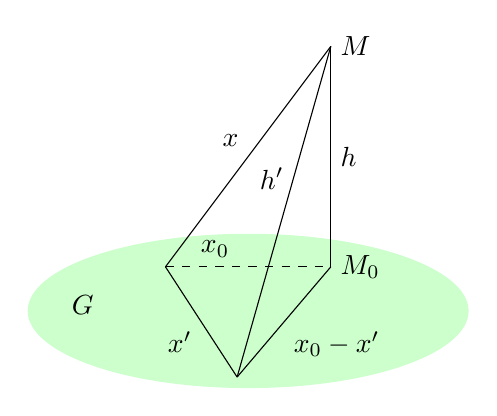
\begin{tikzpicture}[scale = 0.7]
    
    \fill[green!20] (1.5, -0.8) ellipse (4cm and 1.4cm);

    \draw (0, 0) -- (3, 4) node[midway, above left] {\(x\)};
    \draw[dashed] (0, 0) -- (3, 0) node[pos = 0.3, above] {\(x_{0}\)};
    \draw (3, 0) -- (3, 4) node[midway, right] {\(h\)};
    \draw (0, 0) -- (1.3, -2) node[midway, below left] {\(x'\)};
    \draw (1.3, -2) -- (3, 0) node[midway, below right] {\(x_{0} - x'\)};
    \draw (1.3, -2) -- (3, 4) node[pos = 0.6, left] {\(h'\)};

    \draw node[right] at (3, 4) {\(M\)};
    \draw node[right] at (3, 0) {\(M_{0}\)};
    \draw node at (-1.5, -0.7) {\(G\)};

  \end{tikzpicture}
\end{figure}